\documentclass{standalone}

\usepackage{tikz,pgf} %and any other packages or tikzlibraries your picture needs

\begin{document}



\tikzset{every picture/.style={line width=0.75pt}} %set default line width to 0.75pt        

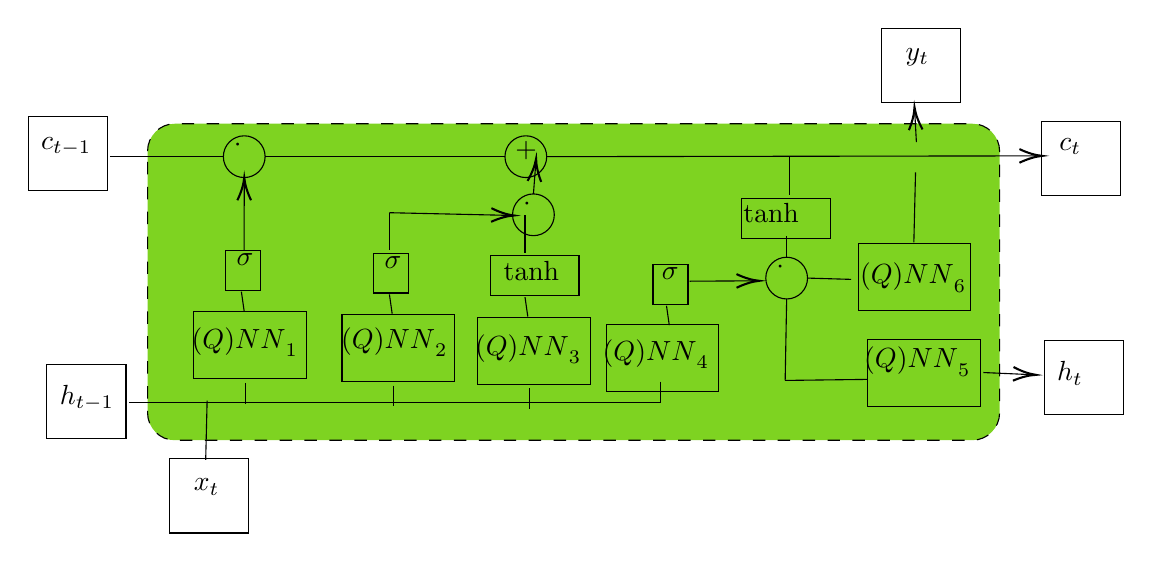
\begin{tikzpicture}[x=0.75pt,y=0.75pt,yscale=-1,xscale=1]
%uncomment if require: \path (0,446); %set diagram left start at 0, and has height of 446

%Rounded Rect [id:dp6392908859797635] 
\draw  [fill={rgb, 255:red, 126; green, 211; blue, 33 }  ,fill opacity=1 ][dash pattern={on 4.5pt off 4.5pt}] (99,111.22) .. controls (99,103.92) and (104.92,98) .. (112.22,98) -- (496.28,98) .. controls (503.58,98) and (509.5,103.92) .. (509.5,111.22) -- (509.5,237.28) .. controls (509.5,244.58) and (503.58,250.5) .. (496.28,250.5) -- (112.22,250.5) .. controls (104.92,250.5) and (99,244.58) .. (99,237.28) -- cycle ;
%Shape: Rectangle [id:dp1869584502273678] 
\draw   (50.5,214) -- (88.6,214) -- (88.6,249.69) -- (50.5,249.69) -- cycle ;
%Shape: Rectangle [id:dp6462060464497075] 
\draw   (41.5,94.5) -- (79.6,94.5) -- (79.6,130.19) -- (41.5,130.19) -- cycle ;
%Shape: Rectangle [id:dp4500179297522413] 
\draw   (109.5,259.5) -- (147.6,259.5) -- (147.6,295.19) -- (109.5,295.19) -- cycle ;
%Straight Lines [id:da6359727152557328] 
\draw    (80.85,113.88) -- (135.52,113.88) ;
%Shape: Circle [id:dp92121227898605] 
\draw   (135.52,113.88) .. controls (135.52,108.33) and (140.02,103.83) .. (145.58,103.83) .. controls (151.13,103.83) and (155.63,108.33) .. (155.63,113.88) .. controls (155.63,119.44) and (151.13,123.94) .. (145.58,123.94) .. controls (140.02,123.94) and (135.52,119.44) .. (135.52,113.88) -- cycle ;
%Straight Lines [id:da08082277368338286] 
\draw    (155.63,113.88) -- (271.19,113.88) ;
%Shape: Circle [id:dp15308340346642546] 
\draw   (271.19,113.88) .. controls (271.19,108.33) and (275.69,103.83) .. (281.24,103.83) .. controls (286.79,103.83) and (291.3,108.33) .. (291.3,113.88) .. controls (291.3,119.44) and (286.79,123.94) .. (281.24,123.94) .. controls (275.69,123.94) and (271.19,119.44) .. (271.19,113.88) -- cycle ;
%Shape: Rectangle [id:dp9759146623319943] 
\draw   (121.33,188.67) -- (175.52,188.67) -- (175.52,220.88) -- (121.33,220.88) -- cycle ;
%Shape: Rectangle [id:dp1514181601501583] 
\draw   (136.67,159) -- (153.52,159) -- (153.52,178.22) -- (136.67,178.22) -- cycle ;
%Straight Lines [id:da09660210007282433] 
\draw    (90.19,232.22) -- (346.19,232.22) ;
%Straight Lines [id:da1840021909403431] 
\draw    (146.19,222.88) -- (146.19,232.88) ;
%Straight Lines [id:da3165443012722071] 
\draw    (144.19,178.88) -- (145.52,188.22) ;
%Straight Lines [id:da03399836801593259] 
\draw    (145.52,158.88) -- (145.57,125.94) ;
\draw [shift={(145.58,123.94)}, rotate = 90.09] [color={rgb, 255:red, 0; green, 0; blue, 0 }  ][line width=0.75]    (10.93,-3.29) .. controls (6.95,-1.4) and (3.31,-0.3) .. (0,0) .. controls (3.31,0.3) and (6.95,1.4) .. (10.93,3.29)   ;
%Shape: Rectangle [id:dp45199903666102115] 
\draw   (192.67,190) -- (246.85,190) -- (246.85,222.22) -- (192.67,222.22) -- cycle ;
%Shape: Rectangle [id:dp3974717053870489] 
\draw   (208,160.33) -- (224.85,160.33) -- (224.85,179.55) -- (208,179.55) -- cycle ;
%Straight Lines [id:da4621245117073174] 
\draw    (217.52,224.22) -- (217.52,234.22) ;
%Straight Lines [id:da9648802152643472] 
\draw    (215.52,180.22) -- (216.85,189.55) ;
%Straight Lines [id:da23355993373386408] 
\draw    (215.52,140.88) -- (273.52,142.17) ;
\draw [shift={(275.52,142.22)}, rotate = 181.27] [color={rgb, 255:red, 0; green, 0; blue, 0 }  ][line width=0.75]    (10.93,-3.29) .. controls (6.95,-1.4) and (3.31,-0.3) .. (0,0) .. controls (3.31,0.3) and (6.95,1.4) .. (10.93,3.29)   ;
%Straight Lines [id:da4127776666064402] 
\draw    (215.52,158.88) -- (215.52,140.88) ;
%Shape: Circle [id:dp47106580719200397] 
\draw   (274.85,141.88) .. controls (274.85,136.33) and (279.36,131.83) .. (284.91,131.83) .. controls (290.46,131.83) and (294.96,136.33) .. (294.96,141.88) .. controls (294.96,147.44) and (290.46,151.94) .. (284.91,151.94) .. controls (279.36,151.94) and (274.85,147.44) .. (274.85,141.88) -- cycle ;
%Straight Lines [id:da7735772960981144] 
\draw    (284.91,131.83) -- (286.04,116.88) ;
\draw [shift={(286.19,114.88)}, rotate = 94.32] [color={rgb, 255:red, 0; green, 0; blue, 0 }  ][line width=0.75]    (10.93,-3.29) .. controls (6.95,-1.4) and (3.31,-0.3) .. (0,0) .. controls (3.31,0.3) and (6.95,1.4) .. (10.93,3.29)   ;
%Shape: Rectangle [id:dp1205535087835905] 
\draw   (258,191.33) -- (312.19,191.33) -- (312.19,223.55) -- (258,223.55) -- cycle ;
%Shape: Rectangle [id:dp7409548464912388] 
\draw   (264.19,161.67) -- (306.85,161.67) -- (306.85,180.88) -- (264.19,180.88) -- cycle ;
%Straight Lines [id:da20145995210827605] 
\draw    (282.85,225.55) -- (282.85,235.55) ;
%Straight Lines [id:da8985206374070698] 
\draw    (280.85,181.55) -- (282.19,190.88) ;
%Straight Lines [id:da03914903084355159] 
\draw    (280.85,160.22) -- (280.85,142.22) ;
%Straight Lines [id:da45949043972455983] 
\draw    (346.19,222.22) -- (346.19,232.22) ;
%Straight Lines [id:da008075800485505713] 
\draw    (408.19,113.72) -- (408.19,132.38) ;
%Shape: Rectangle [id:dp23305246530675738] 
\draw   (385.19,134.17) -- (427.85,134.17) -- (427.85,153.38) -- (385.19,153.38) -- cycle ;
%Straight Lines [id:da590983636135509] 
\draw    (127.69,231.38) -- (127,260) ;
%Shape: Rectangle [id:dp7509434833000515] 
\draw   (320,194.83) -- (374.19,194.83) -- (374.19,227.05) -- (320,227.05) -- cycle ;
%Straight Lines [id:da7966626845205629] 
\draw    (349.02,185.72) -- (350.35,195.05) ;
%Shape: Rectangle [id:dp9672358901977056] 
\draw   (342.5,165.83) -- (359.35,165.83) -- (359.35,185.05) -- (342.5,185.05) -- cycle ;
%Straight Lines [id:da9049778369207253] 
\draw    (360.19,173.88) -- (391.69,173.7) ;
\draw [shift={(393.69,173.69)}, rotate = 179.66] [color={rgb, 255:red, 0; green, 0; blue, 0 }  ][line width=0.75]    (10.93,-3.29) .. controls (6.95,-1.4) and (3.31,-0.3) .. (0,0) .. controls (3.31,0.3) and (6.95,1.4) .. (10.93,3.29)   ;
%Shape: Circle [id:dp1581913184714545] 
\draw   (396.85,172.38) .. controls (396.85,166.83) and (401.36,162.33) .. (406.91,162.33) .. controls (412.46,162.33) and (416.96,166.83) .. (416.96,172.38) .. controls (416.96,177.94) and (412.46,182.44) .. (406.91,182.44) .. controls (401.36,182.44) and (396.85,177.94) .. (396.85,172.38) -- cycle ;
%Straight Lines [id:da2428794509160681] 
\draw    (406.91,152.33) -- (406.91,162.33) ;
%Straight Lines [id:da30267985577469614] 
\draw    (406.91,182.44) -- (406.19,221.69) ;
%Straight Lines [id:da7403458349367105] 
\draw    (406.19,221.69) -- (445.69,221.19) ;
%Shape: Rectangle [id:dp4085004194032973] 
\draw   (446,201.83) -- (500.19,201.83) -- (500.19,234.05) -- (446,234.05) -- cycle ;
%Straight Lines [id:da10833051883144162] 
\draw    (438,173) -- (416.96,172.38) ;
%Straight Lines [id:da3767520354017082] 
\draw    (469,121.5) -- (468.19,155.19) ;
%Shape: Rectangle [id:dp9947916841864535] 
\draw   (441.32,155.83) -- (495.5,155.83) -- (495.5,188.05) -- (441.32,188.05) -- cycle ;
%Straight Lines [id:da6344636492657498] 
\draw    (469.41,106.83) -- (468.61,92) ;
\draw [shift={(468.5,90)}, rotate = 86.91] [color={rgb, 255:red, 0; green, 0; blue, 0 }  ][line width=0.75]    (10.93,-3.29) .. controls (6.95,-1.4) and (3.31,-0.3) .. (0,0) .. controls (3.31,0.3) and (6.95,1.4) .. (10.93,3.29)   ;
%Shape: Rectangle [id:dp07716686492959002] 
\draw   (452.5,52) -- (490.6,52) -- (490.6,87.69) -- (452.5,87.69) -- cycle ;
%Straight Lines [id:da1524470379359495] 
\draw    (501.69,217.88) -- (525,218.91) ;
\draw [shift={(527,219)}, rotate = 182.52] [color={rgb, 255:red, 0; green, 0; blue, 0 }  ][line width=0.75]    (10.93,-3.29) .. controls (6.95,-1.4) and (3.31,-0.3) .. (0,0) .. controls (3.31,0.3) and (6.95,1.4) .. (10.93,3.29)   ;
%Shape: Rectangle [id:dp3090414281277485] 
\draw   (531,202.5) -- (569.1,202.5) -- (569.1,238.19) -- (531,238.19) -- cycle ;
%Shape: Rectangle [id:dp8736519920950074] 
\draw   (529.5,97) -- (567.6,97) -- (567.6,132.69) -- (529.5,132.69) -- cycle ;
%Straight Lines [id:da03755328202040231] 
\draw    (291.3,113.88) -- (528,113.5) ;
\draw [shift={(530,113.5)}, rotate = 179.91] [color={rgb, 255:red, 0; green, 0; blue, 0 }  ][line width=0.75]    (10.93,-3.29) .. controls (6.95,-1.4) and (3.31,-0.3) .. (0,0) .. controls (3.31,0.3) and (6.95,1.4) .. (10.93,3.29)   ;

% Text Node
\draw (55.5,222.9) node [anchor=north west][inner sep=0.75pt]    {$h_{t-1}$};
% Text Node
\draw (46.5,103.4) node [anchor=north west][inner sep=0.75pt]    {$c_{t-1}$};
% Text Node
\draw (120,267.9) node [anchor=north west][inner sep=0.75pt]    {$x_{t}$};
% Text Node
\draw (139.33,104.4) node [anchor=north west][inner sep=0.75pt]    {$\cdot $};
% Text Node
\draw (275,105.07) node [anchor=north west][inner sep=0.75pt]    {$+$};
% Text Node
\draw (140.67,159.4) node [anchor=north west][inner sep=0.75pt]    {$\sigma $};
% Text Node
\draw (212,160.73) node [anchor=north west][inner sep=0.75pt]    {$\sigma $};
% Text Node
\draw (278.67,132.4) node [anchor=north west][inner sep=0.75pt]    {$\cdot $};
% Text Node
\draw (269.33,163.07) node [anchor=north west][inner sep=0.75pt]    {$\tanh$};
% Text Node
\draw (345.5,166.23) node [anchor=north west][inner sep=0.75pt]    {$\sigma $};
% Text Node
\draw (400.67,162.9) node [anchor=north west][inner sep=0.75pt]    {$\cdot $};
% Text Node
\draw (463,60.4) node [anchor=north west][inner sep=0.75pt]    {$y_{t}$};
% Text Node
\draw (536,211.4) node [anchor=north west][inner sep=0.75pt]    {$h_{t}$};
% Text Node
\draw (537,103.9) node [anchor=north west][inner sep=0.75pt]    {$c_{t}$};
% Text Node
\draw (384.83,135.07) node [anchor=north west][inner sep=0.75pt]    {$\tanh$};
% Text Node
\draw (119,194.9) node [anchor=north west][inner sep=0.75pt]    {$\text{(Q)NN}_{1}$};
% Text Node
\draw (191,194.9) node [anchor=north west][inner sep=0.75pt]    {$\text{(Q)NN}_{2}$};
% Text Node
\draw (255.5,198.4) node [anchor=north west][inner sep=0.75pt]    {$\text{(Q)NN}_{3}$};
% Text Node
\draw (317,200.9) node [anchor=north west][inner sep=0.75pt]    {$\text{(Q)NN}_{4}$};
% Text Node
\draw (443,204.4) node [anchor=north west][inner sep=0.75pt]    {$\text{(Q)NN}_{5}$};
% Text Node
\draw (441,163.9) node [anchor=north west][inner sep=0.75pt]    {$\text{(Q)NN}_{6}$};


\end{tikzpicture}

\end{document}